\documentclass{beamer}

%\usetheme{AnnArbor}
%\usetheme{Antibes}
%\usetheme{Bergen}
%\usetheme{Berkeley}
%\usetheme{Berlin}
\usetheme{Boadilla}
%\usetheme{boxes}
%\usetheme{CambridgeUS}
%\usetheme{Copenhagen}
%\usetheme{Darmstadt}
%\usetheme{default}
%\usetheme{Frankfurt}
%\usetheme{Goettingen}
%\usetheme{Hannover}
%\usetheme{Ilmenau}
%\usetheme{JuanLesPins}
%\usetheme{Luebeck}
%\usetheme{Madrid}
%\usetheme{Malmoe}
%\usetheme{Marburg}
%\usetheme{Montpellier}
%\usetheme{PaloAlto}
%\usetheme{Pittsburgh}
%\usetheme{Rochester}
%\usetheme{Singapore}
%\usetheme{Szeged}
%\usetheme{Warsaw}
\usepackage{epsfig}

\usepackage{amssymb, graphicx, amsmath, amsthm}

\usepackage{tikz}
\usetikzlibrary{positioning}
\usetikzlibrary{calc}

\makeatletter
\newcommand*{\rom}[1]{\expandafter\@slowromancap\romannumeral #1@}
\makeatother
\setbeamercovered{highly dynamic}
\newcounter{saveenumi}
\newcommand{\seti}{\setcounter{saveenumi}{\value{enumi}}}
\newcommand{\conti}{\setcounter{enumi}{\value{saveenumi}}}

\title{\textsc{Mathematics for Economics PhD}}


\subtitle{Lecture 2} 
\author{Instructor:  Mariam Arzumanyan}


\date[UIUC, Fall 2021]{University of Illinois at Urbana-Champaign \\August 17, 2021 }


\subject{Lecture Session}

\AtBeginSubsection[]
{
  \begin{frame}<beamer>{Outline}
    \tableofcontents[currentsection,currentsubsection]
  \end{frame}
}
\pgfdeclareimage[height=0.7cm]{Illinilogo}{Illinilogo.png}
\logo{\pgfuseimage{Illinilogo}} 
% Let's get started
\addtobeamertemplate{navigation symbols}{}{%
    \usebeamerfont{footline}%
    \usebeamercolor[fg]{footline}%
    \hspace{1em}%
    \insertframenumber/\inserttotalframenumber
}
\setbeamercovered{invisible}
\begin{document}

\begin{frame}
  \titlepage
\end{frame}

\AtBeginSection[]
{
  \begin{frame}
    \frametitle{Table of Contents}
    \tableofcontents[currentsection]
  \end{frame}
}

\begin{frame}{Class Information}
\begin{itemize}
  
    \item \textbf{Phone:} **
    \item \textbf{Email:} **
\item \textbf{Office Hours:}  1:30 - 2:30 pm  by appointment
\item \textbf{Zoom: } ** 
\item \textbf{During Class:} Please have your Video on and Sound muted. 

\end{itemize}

\end{frame}
\begin{frame}{References}
	\begin{itemize}

\item	\textbf{Simon, Blume, Mathematics for Economists \textit{W.W.Norton, 1994}}
\item	Mas-Colell, Whinston, Green, Microeconomic Theory: Mathematical Appendix \textit{Oxford University Press,  1995 }
\item		Sydsater, Hammond, Seierstad, and Strom, (2008). Further mathematics for economic analysis. Pearson education. Financial Times/Prentice Hall, second edition.
\item		Stokey, Lucas, Prescott, (1989). Recursive Methods in Economics Dynamic, Harvard University Press.

 \end{itemize}   
\end{frame}

\begin{frame}{Topics in Mathematical Analysis}
    \begin{itemize}
        \item A central concern in economic theory is the effect of a small change in one economic variable on some other economic variable. 
        \item Before we can make this effect precise, we need to have a working knowledge of the concepts of \textit{small} and \textit{nearby}. 
        \item This lecture focuses on these questions by studying in some detail the notions of sequence, limit, neighborhood, open sets, closed set, etc.
    \end{itemize}
\end{frame}
\section{Points, Vectors, Lines, Planes}
\begin{frame}{The Real Line}
\begin{itemize}
    \item The simplest geometric object is the number line - the geometric realization of the set of all real numbers. 
    \item Every real number is represented by exactly one point on the line, and each point on the line represents one and only one number.
\end{itemize}
\bigskip

\usetikzlibrary{arrows}
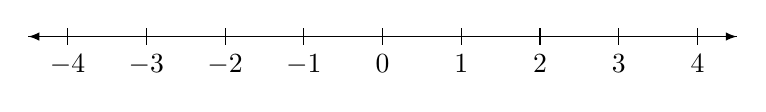
\begin{tikzpicture}
\draw[latex-] (-4.5,0) -- (4.5,0) ;
\draw[-latex] (-4.5,0) -- (4.5,0) ;
\foreach \x in  {-4,-3,-2,-1,0,1,2,3,4}
\draw[shift={(\x,0)},color=black] (0pt,3pt) -- (0pt,-3pt);
\foreach \x in  {-4,-3,-2,-1,0,1,2,3,4}
\draw[shift={(\x,0)},color=black] (0pt,0pt) -- (0pt,-3pt) node[below] 
{$\x$};
\label{The Real Line}
\end{tikzpicture}
\end{frame}


\begin{frame}{Planes}
    \begin{itemize}
        \item In some economic examples, we use pair of numbers to represent economic objects. 
        \item Pairs of numbers also have a geometric representation, called \textbf{Cartesian plane} or \textbf{Euclidean space}, and written as \textbf{$\mathbb{R}^2$}.
      \item   To depict $\mathbb{R}^2$, we draw two perpendicular number lines: one horizontal to represent the first component, and the other vertical to represent the second component. 
      \item These two number lines are called \textbf{coordinate axes}. They intersect at their \textbf{origins}.
      \item A point $p$ or vector  in the Cartesian plane represents a pair of numbers $(a, b)$.
    \end{itemize}
\end{frame}
\begin{frame}{Three Dimension and More}
\begin{itemize}
    \item We can visualize $3$-dimensional Euclidean space $\mathbb{R}^3$ by drawing three mutually perpendicular number lines. 
    \item Each of these lines is called a \textbf{coordinate axis}. Each point or vector is represented by the triple $(a,b,c).$ 
    \item Similarly, Euclidean $n$-space is usually referred as $\mathbb{R}^n$. The number $n$ refers to how many numbers are needed to describe each point. 
\end{itemize}
    
%\end{item}
    
\end{frame}


\begin{frame}{Length and Distance}
\begin{itemize}
    \item If $P=(a_1,a_2,...,a_n)$ and $Q=(b_1, b_2,..., b_n)$ are two points in Euclidean space $\mathbb{R}^n$, we write $PQ$ for the line segment joining $P$ to $Q$ and $\vec{PQ}$ for the vector from $P$ to $Q$. 
    
\end{itemize}
\begin{block}{Definition}
    The \textbf{length} of line segment $PQ$ is denoted by $\lvert\lvert PQ\rvert \rvert $, and it is equal:
    \[\lvert\lvert PQ\rvert \rvert =\sqrt{(b_1-a_1)^2+(b_2-a_2)^2+\cdots+(b_n-c_n)^2}.
    \]
\end{block}
    \begin{itemize}
        \item The distance from the point $x=(x_1, x_2,...,x_n)$ to the origin or the \textbf{length } of vector $\vec{x}$ is 
        \[\lvert\lvert \vec{x}\rvert \rvert= \sqrt{x_1^2+...+x_n^2}.
        \]
        \item $\lvert\lvert r \vec{v}\rvert \rvert= |r|\lvert\lvert \vec{v}\rvert \rvert$ for all real $r$ and $v\in \mathbb{R}^n$.
    \end{itemize}
    \end{frame}


\begin{frame}{The Inner Product}
\begin{block}{Definition}
Let $\vec{u}=(u_1,..., u_n)$ and $\vec{v}=(v_1,..., v_n)$ be two vectors in $\mathbb{R}^n$. The \textbf{Euclidean inner product} of $\vec{u}$ and $\vec{v}$, written $\vec{u}\cdot\vec{v}$, is the number
\[\vec{u}\cdot\vec{v}=u_1v_1+u_2v_2+...+u_nv_n.
\]
Euclidean inner product os often called the \textbf{dot product} or the \textbf{scalar product.}
\end{block}
Let $\vec{u}$, $\vec{v}$, and $\vec{w}$ be arbitrary vectors in $\mathbb{R}^n$ and let $r$ be an arbitrary scalar. Then,
\begin{enumerate}
    \item $\vec{u}\cdot\vec{v}=\vec{v}\cdot\vec{u}$.
    \item $\vec{u}\cdot(\vec{v}+\vec{w})=\vec{u}\cdot\vec{v}+\vec{u}\cdot\vec{w}$.
    \item $\vec{u}\cdot(r\vec{v})=r(\vec{u}\cdot\vec{v})=(r\vec{u})\cdot\vec{v}$.
    \item $\vec{u}\cdot\vec{u}\geq 0$, and $\vec{u}\cdot\vec{u}=0$ if and only if $\vec{u}=0$.
\end{enumerate}
 \end{frame}


\begin{frame}{The Inner Product}
\begin{itemize}
    \item The Euclidean inner product is closely connected to the Euclidean length of a vector. 
    
\end{itemize}
\begin{block}{Theorem}
Let $\vec{u}$ and $\vec{v}$ be two vectors in $\mathbb{R}^n$. Let $\theta$ be the angle between them. Then, 
\[\vec{u}\cdot\vec{v}=||u||||v||\cos{\theta}
\]
\end{block}
This implies that the angle between vectors $\vec{u}$ and $\vec{v}$ in $\mathbb{R}^n$ is 
\begin{itemize}
    \item acute, if $\vec{u}\cdot\vec{v}>0$,
    \item obtuse, if $\vec{u}\cdot\vec{v}<0$, 
    \item right, if $\vec{u}\cdot\vec{v}=0$, in which case we say that $\vec{u}$ and $\vec{v}$ are \textbf{orthogonal.}
\end{itemize}
\end{frame}

\begin{frame}{The Inner Product}
\begin{block}{Triangle Inequality}
For any two vectors $\vec{u}$ and $\vec{v}$ in $\mathbb{R}^n$,
\[||u+v||\leq ||u||+||v||,
\]
and 
\[||u||-||v||\leq ||u-v||.
\]
\end{block}

    
\end{frame}

\begin{frame}{Lines}
    \begin{itemize}
        \item First, we will work with lines in $\mathbb{R}^2$. Straight line have an equation of the form
        \[y=ax+b.
        \]
        \item The coefficient $a$ is the slope of the line and the coefficient $b$ is the $y$-intercept.
        \item We will often find a parametric representation of the line more useful.The \textbf{line segment joining} $\vec{u}$ to $\vec{v}$ is 
        \[  l(\vec{u}, \vec{v})=\{(1-t)\vec{u}+t\vec{v}:0\leq t\leq 1\}
        \]
        \item The most famous example is \textbf{budget line}
        \[p_xx+p_yy=w, \text{ or } \{(1-t)\frac{w}{p_x}+t\frac{w}{p_y}: 0\leq t\leq 1\}.
        \]
    \end{itemize}
\end{frame}
\section{Basis and Dimensions}
\begin{frame}{Linear Independence}
    \begin{block}{Definition}
    Vectors $\vec{v}_1,\vec{v}_2,\cdots, \vec{v}_k$ in $\mathbb{R}^n$ are \textbf{linearly dependent} if and only if there exist scalars $c_1,c_2, \cdots , c_k$ not all zero, such that 
    \[c_1v_1+c_2v_2+\cdots+c_kv_k=0.
    \]
    
    Vectors $\vec{v}_1,\vec{v}_2,\cdots, \vec{v}_k$ in $\mathbb{R}^n$ are \textbf{linearly independent} if and only if $c_1v_1+c_2v_2+\cdots+c_kv_k=0$ for scalars $c_1,c_2, \cdots , c_k$ implies that  $c_1=c_2=\cdots =c_k=0$.
    \end{block}
    The vectors 
    
    \begin{align*}
        \begin{array}{ccc}
           e_1 =\begin{pmatrix}
           1\\ 0\\ \vdots \\0
           \end{pmatrix},& \cdots   
             & e_n =\begin{pmatrix}
           0\\ 0\\ \vdots \\1
           \end{pmatrix}
        \end{array}
    \end{align*}
    in $\mathbb{R}^n$ are \textbf{linearly independent}.
\end{frame}

\begin{frame}{Linear Independence}
\begin{block}{Theorem}
Vectors $\vec{v}_1,\vec{v}_2,\cdots, \vec{v}_k$ in $\mathbb{R}^n$ are linearly dependent if and only if the linear system 
\[A\begin{pmatrix}
c_1\\ \vdots \\ c_k \end{pmatrix}=0
\]
has a nonzero solution $(c_1,\cdots, c_k)$, where $A$ is the $n\times k$ matrix whose columns are the vectors $\vec{v}_1,\vec{v}_2,\cdots, \vec{v}_k$:
\[A=\begin{pmatrix}
\vec{v}_1 &\vec{v}_2 & \cdots & \vec{v}_k \end{pmatrix}.
\]
\end{block}
\begin{block}{Theorem}
If $k>n$, any set of $k$ vectors in $\mathbb{R}^n$ is linearly dependent.
\end{block}
\end{frame}

\begin{frame}{Linear Independence}
\begin{block}{Theorem}
Vectors $\vec{v}_1,\vec{v}_2,\cdots, \vec{v}_k$ in $\mathbb{R}^n$ are linearly independent if and only if
\[det\begin{pmatrix}
\vec{v}_1 &\vec{v}_2 & \cdots & \vec{v}_k \end{pmatrix}\neq 0.
\]
\end{block}
\end{frame}

\begin{frame}{Basis}
\begin{block}{Theorem}
Let $\vec{v}_1,\vec{v}_2,\cdots, \vec{v}_n$ be a collection of $n$ vectors in $\mathbb{R}^n$. Form $n\times n $ matrix $A=\begin{pmatrix}
\vec{v}_1 &\vec{v}_2 & \cdots & \vec{v}_k \end{pmatrix}$.Then, the following statements are equivalent:
\begin{enumerate}
    \item $\vec{v}_1,\vec{v}_2,\cdots, \vec{v}_n$ are linearly independent, 
    \item $\vec{v}_1,\vec{v}_2,\cdots, \vec{v}_n$ form a basis of $\mathbb{R}^n$, and
    \item the determinant of A is nonzero.
\end{enumerate}
\end{block}
\begin{itemize}
    \item Every basis of $\mathbb{R}^n$ contains $n$ vectors. 
    \item The vectors   
    \begin{align*}
        \begin{array}{ccc}
           e_1 =\begin{pmatrix}
           1\\ 0\\ \vdots \\0
           \end{pmatrix},& \cdots   
             & e_n =\begin{pmatrix}
           0\\ 0\\ \vdots \\1
           \end{pmatrix}
        \end{array}
    \end{align*}
    form a basis in $\mathbb{R}^n$, which is called the \textbf{canonical basis} of $\mathbb{R}^n$.
\end{itemize}
\end{frame}

\section{Limits and Sequences}
\begin{frame}{Limits and Sequences of Real Numbers}
    \begin{block}
{Definition} 
The natural numbers-also called positive integers are just the usual counting numbers: $1,2,3,...$. A \textbf{sequence } of real numbers is an assignment of a real number to each natural number. A sequence is usually written as $\{x_1, x_2, x_3,..., x_n,...\}$, where $x_1$ is the real number assigned to the natural number 1, the first member in the sequence; $x_2$ is the real number assigned to 2, the second member; and so on. 

    \end{block}
    \textbf{Example:} Some examples of sequences of real numbers are:
    \[\{1,2,3,4,...\}, \text{ or } \{1, \frac{1}{2}, \frac{1}{3}, \frac{1}{4},...\},
    \]
    \[\{1, \frac{1}{2}, 4, \frac{1}{8}, 16,...\}, \text{ or } \{ 0, -\frac{1}{2}, \frac{2}{3}, -\frac{3}{4}, \frac{4}{5},...\}
    \]
        
\end{frame}
\begin{frame}{Limits of a Sequence}
\begin{block}{Definition}
Let $\{x_1, x_2, x_3,..., x_n,...\}$ be a sequence of real numbers and let $r$ be a real number. We say that $r$ is the \textbf{limit} of this sequence if for any small positive number $\varepsilon$ there is a positive integer $N$ such that for all $n\geq N$,
\[|x_n-r|<\varepsilon.
\]
In case the sequence converges to $r$, we write 
\[\lim x_n=r \text{ or } \lim_{n\to \infty}x_n=r \text{ or }x_n\to r.
\]
\end{block}
\begin{block}{Theorem}
A sequence can have at most one limit. 
\end{block}        
\end{frame}
\begin{frame}{Limits of a Sequence}
\begin{block}{Theorem}
Let $\{x_n\}_{n=1}^\infty$ and $\{y_n\}_{n=1}^\infty$ be sequences with limits $x$ and $y$. Then the sequence $\{x_n+y_n\}_{n=1}^\infty$ converges to the limit $x+y$.
\end{block}
\begin{block}{Theorem}
Let $\{x_n\}_{n=1}^\infty$ and $\{y_n\}_{n=1}^\infty$ be sequences with limits $x$ and $y$. Then the sequence of products $\{x_ny_n\}_{n=1}^\infty$ converges to the limit $xy$.
\end{block}
\begin{block}{Theorem}
Let $\{x_n\}_{n=1}^\infty$ be a convergent  sequence with limit $x$, and let $b$ be a number such that $x_n\leq b$ (or $x_n\geq b$) for all $n$. Then  the limit $x\leq b$ (or $x_n\geq b$).
\end{block}
\end{frame}

\begin{frame}{Sequences in $\mathbb{R}^m$}
    \begin{itemize}
        \item \textbf{A sequence} in $\mathbb{R}^m$ is what we would expect: an assignment of a vector in $\mathbb{R}^m$ to each natural number n: $\{\vec{x_1}, \vec{x_2},\vec{x_3},\cdots\}$.  
        \begin{block}{Definition}
            Let $\vec{r}$ be a vector in $\mathbb{R}^m$ and let $\varepsilon$ be a positive number. The $\varepsilon$-\textbf{ball about vector }$\vec{r} $ is 
            \[B(\vec{r})=\{\vec{x}\in \mathbb{R}^m: ||\vec{x}-\vec{r}||<\varepsilon\}.\
            \]
        \end{block}
        \item Intuitively, a vector $\vec{x}$ in $\mathbb{R}^m$ \textbf{is close to} $\vec{r}$ if $\vec{x} $ is in some ball $B(\vec{r})$ for a small but positive $\varepsilon$.
    \end{itemize}
    \end{frame}

\begin{frame}{Limits of Sequences in $\mathbb{R}^m$}
\begin{block}
{Definition} A sequence of vectors $\{\vec{x}_n\}_{n=1}^\infty$ is said to converge to the vector $\vec{x}$ if for any choice of a positive real number $\varepsilon$, there is an integer $N$ such that for all $n\geq N$, $\vec{x}_n\in B(\vec{x})$: that is,
\[||\vec{x_n}-\vec{x}||<\varepsilon.
\]
The vector $\vec{x}$ is called the \textbf{limit} of the sequence. 
\end{block}
\begin{block}
{Theorem} A sequence of vectors in $\mathbb{R}^m$ converges if and only of all $m$ sequences of its components converge in $\mathbb{R}^1$.
\end{block}
  \end{frame}

\begin{frame}{Limits of Sequences in $\mathbb{R}^m$}
\begin{block}
{Theorem}
Let $\{\vec{x}_n\}_{n=1}^\infty$, and $\{\vec{y}_n\}_{n=1}^\infty$, be convergent sequences of vectors in $\mathbb{R}^m$ with limits $\vec{x}$ and $\vec{y}$, respectively; and let $\{c_n\}_{n=1}^\infty$ be a convergent sequence of real numbers with limit $c$. Then the sequence $\{c_n\vec{x}_n+\vec{y}_n\}_{n=1}^\infty$ converges to limit $c\vec{x}+\vec{y}$. 
\end{block}
\begin{block}{Definition}
A sequence $\{\vec{y}_j\}_{j=1}^\infty$ of vectors in $\mathbb{R}^m$ is a \textbf{subsequence } of $\{\vec{x}_n\}_{n=1}^\infty$ in $\mathbb{R}^m$ if there exists an infinitely increasing set of natural numbers $\{n_j\}_{j=1}^\infty$ with 
\[n_1<n_2<n_3<...,
\]
such that $\vec{y}_1=\vec{x}_{n_1}$, $\vec{y}_2=\vec{x}_{n_2}$, $\vec{y}_3=\vec{x}_{n_3}$, and so on.
\end{block}

\end{frame}
\section{Open Sets}
\begin{frame}{Open Sets}
\begin{itemize}
    \item For a vector $\vec{z}\in \mathbb{R}^m$ and a positive number $\varepsilon$, the $\varepsilon$-ball about $\vec{z}$ is $B_\varepsilon(\vec{z})=\{\vec{x}\in \mathbb{R}^m: ||\vec{x}-\vec{z}||<\varepsilon\}$.
\end{itemize}
    \begin{block}{Definition}
    A set $S$ in $\mathbb{R}^m$ is \textbf{open} if for each $\vec{x}\in S$, there exists an open $\varepsilon$-ball around $\vec{x}$ completely contained in $S$:
    
    \[\vec{x}\in S \Rightarrow \exists \varepsilon>0 \text{ such that }B_\varepsilon(\vec{x})\subset S.
    \]
    \end{block}
    \begin{itemize}
        \item Any union of open sets is open. 
        \item The \textit{finite} intersection of open sets is open. 
    \end{itemize}
\end{frame}
\begin{frame}{Interior of a Set}
\begin{block}{Definition}
Suppose that $S$ is a subset of $\mathbb{R}^m$. Let $int(S)$ denote the union of all open sets contained in $S$, and it is called the \textbf{interior } of $S$.
\end{block}
\begin{itemize}
    \item By definition, the interior of  a set can be considered as the largest open set which is contained in the given set. 
    \item The interior of an open set $S$ is the set $S$ itself.
\end{itemize}
    
\end{frame}
\section{Closed Sets}
\begin{frame}{Closed Sets}
    \begin{block}{Definition}
    A set $S$ in $\mathbb{R}^m$ is \textbf{closed} if, whenever $\{\vec{x}_n\}_{n=1}^\infty$ is a convergent sequence completely in $S$, its limit is also contained in $S$.
    \end{block}
    \begin{itemize}
        \item A closed set must contain all its "boundary points", just the opposite of the situation with the open sets. 
        \item A set $S$ is closed if and only if its complement $S^c$ is open. 
        \item Any intersection of closed sets is closed. 
        \item The finite union of closed sets is closed. 
    \end{itemize}
\end{frame}

\begin{frame}{Closure of a Set}
\begin{block}{Definition}
Suppose that $S$ is  a subset of $\mathbb{R}^m$. The \textbf{closure} of $S$ is the intersection of all closed sets containing $S$. 
\end{block}
    \begin{itemize}
        \item By definition, the closure of $S$ is the smallest set which contains $S$. 
        
    \end{itemize}
    \begin{block}{Theorem}
    Let $S $ be a set in $\mathbb{R}^1$. Then $x$ is in closure of $S$ if and only if there is a sequence of points in $S$ converging to $x$. 
    \end{block}
\end{frame}

\begin{frame}{Boundary}
    \begin{block}{Definition}
    A point $x$ is in the \textbf{boundary } of a set $S$ if every open ball about $x$ contains both points in $S$ and in the complement of $S$. 
    \end{block}
    \begin{block}{Theorem}
    The set of boundary points of a set $S$ is the intersection of its closure and the complement of closure. 
    \end{block}
\end{frame}


\begin{frame}{Compact Sets}
    \begin{itemize}
        \item Recall that a set $S\in \mathbb{R}^m$ if $S$ is contained in some ball. 
    \end{itemize}
    \begin{block}{Definition}
    A set $S\in \mathbb{R}^m$ is \textbf{compact} if and only if it is both closed and bounded.  
    \end{block}
    \begin{block}{Bolzano-Weierstrass Theorem}
    Any sequence contained in the compact subset of $\mathbb{R}^m$ has a convergent subsequence. Also, if $S\subset \mathbb{R}^m$ has the property that any sequence in $S$ has a convergent subsequence with its limit in S, then S is closed and bounded.  
    
    
    \end{block}
\end{frame}
\section{Convex Sets}

\begin{frame}{Convex Sets}
    \begin{block}{Definition}
    The set $S\subset \mathbb{R}^m$ is \textbf{convex} if $\alpha x+(1-\alpha)y\in S$ for all $x, y\in S$ and $\alpha\in [0,1]$. 
    
    \end{block}
    \begin{itemize}
        \item In other words: A set in $\mathbb{R}^m$ is convex if whenever it contains two vectors, it also contains the entire segment connecting them. 
        \item The intersection of any number of convex sets is convex, but the union of the convex sets might not be convex. 
        
    \end{itemize}
    \begin{block}{Definition}
    Given a set  $S\subset \mathbb{R}^m$, the \textbf{convex hull} of $S$ is the smallest convex set containing $S$, that is, the intersection of all convex sets that contain $S$:
    \[\{\sum_{j=1}^J\alpha_j x_j: \text{ for some } x_1,..., x_J\in S, \text{ and }\alpha_1,..., \alpha_J\geq 0 \text{ with } \sum_{j=1}^J\alpha_j=1\}.
    \]
    \end{block}
\end{frame}
\begin{frame}{Extreme Points}
    \begin{block}{Definition}
    The vector $x\in S$ is an \textbf{extreme point} of the convex set $S\subset \mathbb{R}^m$ if it cannot be expressed as $x=\alpha z+(1-\alpha)y$ for any $y,z\in S$ and $\alpha\in (0,1)$.
    \end{block}
    \begin{block}{Theorem}
    Suppose that $S\subset \mathbb{R}^m$ is a convex set that is also compact. Then, every $x\in S$ can be expressed as a convex combination of at most $m+1$ points of $S$.
    \end{block}
    \begin{itemize}
        \item This result is extremely powerful when dealing with probability simplex, and in game theory.
    \end{itemize}
\end{frame}

\begin{frame}{Separating Hyperplane Theorems}
    \begin{block}{Definition}
Given $\vec{p}\in \mathbb{R}^m$ with $\vec{p}\neq 0$ and $c\in \mathbb{R}$, the \textbf{hyperplane generated by $\vec{p}$ and $c$}   is the set $H_{p,c}=\{\vec{z}\in \mathbb{R}^m:\vec{p}\cdot \vec{z}=c\} $. The sets $\{\vec{z}\in \mathbb{R}^m:\vec{p}\cdot \vec{z}\geq c\} $ and $\{\vec{z}\in \mathbb{R}^m:\vec{p}\cdot \vec{z}\leq c\} $ are called, respectively, the \textbf{half-space above} and the \textbf{half-space below }the hyperplane. 
    \end{block}
    \begin{block}{Separating Hyperplane Theorem}
    Suppose $S\subset \mathbb{R}^m$ is convex and closed, and that $\vec{x}\notin S$. Then there is $\vec{p}\in \mathbb{R}^m$ with $\vec{p}\neq 0$ and $c\in \mathbb{R}$ such that $\vec{p}\cdot \vec{x}>c$ and $\vec{p}\cdot \vec{y}<c$ for all $\vec{y}\in S$. More generally, suppose that the convex sets $A, B\subset \mathbb{R}^m$ are disjoint (i.e., $A\cap B=\emptyset$). Then, there is a hyperplane that separates A and B, leaving $A$ and $B$ on different sides of it. 
    \end{block}
\end{frame}
\section{Functions}
\begin{frame}{Functions}
   \begin{block}{Definition} A \textbf{function} from set $A$ to set $B$ is a rule that assigns to each object in A, one and only one object in $B$. In this case, we write $f:A\to B$. Then, $A$ is the \textbf{domain } of $f$ and $B$ is the \textbf{target space} of $f$. If $C\subset A$, then the \textbf{image} of $C$ under $f$ is 
   \[f(C)=\{b\in B:b=f(a) \text{ for some }a \in C\}. 
   \]
   On the other hand, if $V$ is a subset of the target space $B$, then the \textbf{preimage} of $V$ under $f$ is the set of all points in the domain whose image lies in $V$:
   \[f^{-1}(V)=\{a\in A: f(a)\in V\}.
   \]
   \end{block}
   
  \end{frame}

\begin{frame}{Functions}
Consider the function $f:A\to B$. Let $U_1$ and $U_2$ be arbitrary subsets of the domain $A$, and let $V_1$ and $V_2$ be arbitrary subsets of the target space $B$. 

\begin{itemize}
    \item If $U_1\subset U_2$, $f(U_1)\subset f(U_2)$.
    \item If $V_1 \subset V_2$, $f^{-1}(V_1)\subset f^{-1}(V_2)$.
    \item For all sets $U$, $U\subset f^{-1}(f(U))$.
    \item For all sets $V$, $f(f^{-1}(V))\subset V$.
    \item For all sets $V$, $f^{-1}(V^c)=(f^{-1}(V))^c$.
\end{itemize}
  \end{frame}

\begin{frame}{ Functions}
\begin{itemize}
    \item If for each element $b\in B$ there is an element $a\in A$ such that $b=f(a)$, we say that $f$ maps A \textbf{onto } $B$ or that $f$ is \textbf{surjective}. 
    \item A function $f$ is \textbf{one-to-one} or \textbf{injective} on a subset $C$ of $A$ if and only if for every $x, y$ in $C$
    \[f(x)=f(y) \Rightarrow x=y.
    \]
    \item When $f:A\to B $ is one-to-one on a set $C\subset A$, then there is an \textbf{inverse function} of $f$ on $C$ and is written as:
    \[f^{-1}:f(C)\to C.
    \]
    \item Let $f:A \to B$ and $g:C \to D$ be two functions. Suppose that $B$, the image of $f$, is a subset of C, the domain of $g$. Then, the \textbf{composition} of $f$ with $g$, $g\circ f:A \to D$, is defined the function
    \[(g\circ f)(x)=g(f(x)) \text{ for all } x\in A.
    \]
\end{itemize}
\end{frame}

\begin{frame}{Continuous Functions}
\begin{block}{Definition}
A function $f:A\to B$ is \textbf{continuous} at $x_0\in A$ if for any sequence $\{x_n\}_{n=1}^\infty$ which converges to $x_0$ in $A$, $f(x_n)$ converges to $f(x_0)$. A function is \textbf{continuous on a set} $C\subset A$ if it is continuous at every $x\in C$. Finally, we say that a function is continuous if it is continuous at every point in its domain. 
\end{block}
Suppose that $f:X\to \mathbb{R}^k$ is a continuous function defined on a nonempty set $X\subset \mathbb{R}^m$. 
\begin{enumerate}
    \item The image of a compact set under $f(\cdot)$ is compact. That is, if $A\subset X$ is compact, then $f(A)$ is a compact subset of $\mathbb{R}^k$.
    \item Suppose $k=1$ and $X$ is compact. Then $f(\cdot )$ has a maximizer. That is, there is $x\in X$ such that $f(x)\geq f(x')$ for every $x'\in X$.
\end{enumerate}
\end{frame}

\begin{frame}{Weierstrass's Theorem}
\begin{block}{Theorem}
Let $F:C\to \mathbb{R}^1$ be a continuous function whose domain is a compact subset $C$ in $\mathbb{R}^n$. Then, there exist points $x_m$ and $x_M$ in $C$ such that $F(x_m)\leq F(x)\leq F(x_M)$ for all $x\in C$; that is, $x_m\in C$ is the global min of $F$ in $C$ and $x_M$ is the global max of $F$ in $C$.
\end{block}
    
\end{frame}
\section{Derivatives}

\begin{frame}{Differentiable Functions}
Let's start with functions of one-variable
\begin{block}{Definition}
A function $f:A\to B$ is \textbf{differentiable} at $x_0\in A$ if for any sequence $\{x_n\}_{n=1}^\infty$ which converges to $x_0$ in $A$, 
\[
f'(x_0)=\lim_{n\to \infty}\frac{f(x_n)-f(x_0)}{x_n-x_0}
\]
if this limit exists. A function is \textbf{differentiable on a set} $C\subset A$ if it is differentiable at every $x\in C$. Finally, we say that a function is differentiable if it is differentiable at every point in its domain.
\end{block}
\end{frame}
\begin{frame}{Rolle's Theorem and Mean Value Theorem}
    \begin{block}{Rolle's Theorem}
    Suppose that $f:[a,b]\to \mathbb{R}^1$ is continuous differentiable. If $f(a)=f(b)=0$, then there exists a point $c\in (a, b)$ such that $f'(c)=0$.
    \end{block}
     \begin{block}{Mean Value Theorem}
   Let  $f:U\to \mathbb{R}^1$ be a  continuous differentiable function on a connected interval $U$ in $\mathbb{R}^1$. For any points $a, b \in U$, there is a point $c$ between $a$ and $b$ so that 
   \[f(b)-f(a)=f'(c)(b-a).
   \]
    \end{block}
\end{frame}

\begin{frame}{Taylor Polynomials}
    \begin{block}{Definition}
    The \textbf{$k$th order Taylor polynomial} of $f$ at $x=a$ is 
    \[P_k(a+h)=f(a)+f'(a)h+\frac{1}{2! }f"(a)h^2+\cdots +\frac{1}{k!}f^{[k]}(a)h^k.
    \]
    \end{block}
    \begin{block}{Theorem}
     Let  $f:U\to \mathbb{R}^1$ be a $(k+1)$ times continuously differentiable function on a connected interval $U$ in $\mathbb{R}^1$. For any points $a, a+h \in U$, there is a point $c^*$ between $a$ and $a+h$ such that 
     \[f(a+h)=f(a)+f'(a)h+\frac{1}{2! }f"(a)h^2+\cdots\]
     \[+\frac{1}{k!}f^{[k]}(a)h^k+\frac{1}{(k+1)!}f^{k+1}(c^*)h^{k+1}.
     \]
    \end{block}
\end{frame}


\begin{frame}{Computing Derivative}
Suppose that $\alpha$ is an arbitrary constant and $f$ and $g$ are differentiable functions. Then, 
    \begin{itemize}
        \item $(f\pm g)'(x)=f'(x)+g'(x)$,
        \item $(\alpha f)'(x)=\alpha f'(x)$, 
        \item $(f\cdot g)'(x)=f'(x)g(x)+f(x)g'(x)$,
        \item $(\frac{f}{g})'(x)=\frac{f'(x)g(x)-f(x)g'(x)}{g^2(x)}$,
        \item $(( f(x))^\alpha)'=\alpha(f(x))^{\alpha-1}\cdot f'(x)$,
        \item $(x^\alpha)'=\alpha x^{\alpha-1}$.
    \end{itemize}
\end{frame}

\begin{frame}{Exponential Functions}
    \begin{itemize}
        \item Functions in which the variable $x$ appears as an exponent are called \textbf{exponential functions}. 
        \item For example, $f(x)=2^x$ is an exponential function and the number 2 is called the \textbf{base} of the exponential function. 
        \item If $x$ is a positive integer, $2^x$ means multiply 2 by itself $x $ times. 
        \item If $x=\frac{1}{n}$, $2^x=\sqrt[n]{2}$, the $n$th root of 2. 
        \item If $x=\frac{m}{n}$, $2^{\frac{m}{n}}=(\sqrt[n]{2})^m$, the $m$th power of the $n$th root of 2. 
        \item If $x$ is a negative number, $2^x$ means $\frac{1}{2^{|x|}}$, the reciprocal of $2^{|x|}$.
    \end{itemize}
    \end{frame}

\begin{frame}{Exponential Functions}
\begin{itemize}
    \item The number $e$ plays very fundamental role in economics. It is defined formally:
    \[e=\lim_{n\to \infty }(1+\frac{1}{n})^n,
    \]
    and it is approximately equal to $e=2.7182818.$
    \item The function $f(x)=e^x$ is called \textbf{the exponential function} and is frequently written as $\exp(x)$
\end{itemize}
\end{frame}

\begin{frame}{Logarithm Functions}
\begin{itemize}
    \item The \textbf{logarithm }of $x$ is the power to which one must raise $a$ to yield $x$:
    \[a^{\log_{a}{x}}=x \text{ and }\log_{a}{a^x}=x.
    \]
    \item We call $a$ the \textbf{base of the logarithm}. The most famous cases are when $a=10$ and $a=e$. 
    \item The $\log_ex$ is the inverse of the $e^x$ exponential function. It is called \textbf{natural logarithm} function and denoted by $\ln x$:
    \[\ln x=y \iff e^y=x, \text{ and }e^{\ln x}=x \text{ and } \ln e^x=x.
    \]
    
\end{itemize}
    
\end{frame}
\begin{frame}{Properties of Exp and Log}
\begin{enumerate}
    \item $a^r\cdot a^s=a^{r+s}$, and $\log (r\cdot s)=\log r+\log s$.
    \item $a^{-r}=\frac{1}{a^r}$, and $\log (\frac{1}{r})=-\log r. $
    \item $\frac{a^r}{a^s}=a^{r-s}$, and $\log (\frac{r}{s})=\log r -\log s$.
    \item $(a^r)^s=a^{rs}$, and $\log r^s=s \log r$. 
    \item $a^0=1$, and $\log 1=0$.
\end{enumerate}
    
\end{frame}

\begin{frame}{Derivatives of Exp and Log}
\begin{block}{Theorem}
The functions $e^x$ and $\ln x$ are continuous functions on their domains and have continuous derivatives of every order. Their first derivatives are given by 
\[(e^x)'=e^x
\] and 
\[(\ln x)'=\frac{1}{x}.
\]
If $u(x)$ is a differentiable function, then 
\[(e^{u(x)})'=(e^{u(x)})u'(x), 
\]
 and 
 \[(\ln u(x))'=\frac{u'(x)}{u(x)} \text{ if } u(x)>0.
 \]
 For any fixed base $a$, 
 \[(a^x)'=\ln a (a^x).
 \]
\end{block}
    
\end{frame}

\begin{frame}{Partial Derivatives}
Suppose we are looking at the function $y=f(x_1, x_2,..., x_k)$.
\begin{block}{Definition}
Let $f:\mathbb{R}^k\to \mathbb{R}$. Then, for each variable $x_i$ at point $x_0=(x_1^0,..., x_n^0)$ in the domain of $f$, 
\[\frac{\partial f}{\partial x_i} (x_1^0,..., x_n^0)=\lim_{h\to 0}\frac{f(x_1^0,..., x_i^0+h,..., x_n^0)-f(x_1^0,..., x_i^0,..., x_n^0) }{h}
\]
if the limit exists. Only the $i$th variable changes, the others are treated as constants. The matrix 
\[[\nabla f(x)]^T=Df(x)=\begin{pmatrix} \frac{\partial f}{\partial x_1}(x) & \cdots & \frac{\partial f}{\partial x_k}(x)\end{pmatrix}
\] represents the transpose of the \textbf{gradient} vector of $f$ at $x$, or sometimes the \textbf{Jacobian derivative} of $f$ at $x$.
\end{block}
    \end{frame}

\begin{frame}{Partial Derivatives}
\begin{block}{Definition}
Let $f:\mathbb{R}^k\to \mathbb{R}^m$. 
 The matrix 
\[Df(x)=\begin{pmatrix} \frac{\partial f_1}{\partial x_1}(x) & \frac{\partial f_1}{\partial x_2}(x)& \cdots & \frac{\partial f_1}{\partial x_k}(x)\\
\vdots & \vdots &\ddots & \vdots\\
 \frac{\partial f_m}{\partial x_1}(x) & \frac{\partial f_1}{\partial x_2}(x)& \cdots & \frac{\partial f_m}{\partial x_k}(x)\\
\end{pmatrix}
\] represents the \textbf{derivative}  of $f$ at $x$, or the \textbf{Jacobian derivative} of $f$ at $x$.
\end{block}
\end{frame}

\begin{frame}{Hessian Matrix}
\begin{block}{Definition}
Let $f:\mathbb{R}^k\to \mathbb{R}$. 
 The matrix 
\[D(\nabla f(x))=D^2f(x)=\begin{pmatrix} \frac{\partial^2 f}{\partial x_1^2}(x) & \frac{\partial^2 f}{\partial x_1\partial x_2}(x)& \cdots & \frac{\partial^2 f}{\partial x_1\partial x_k}(x)\\
\vdots & \vdots &\ddots & \vdots\\
 \frac{\partial^2 f}{\partial x_k\partial x_1}(x) & \frac{\partial^2 f}{\partial x_k \partial x_2}(x)& \cdots & \frac{\partial^2 f}{\partial x_k^2}(x)\\
\end{pmatrix}
\] represents the \textbf{ second derivative}  of $f$ at $x$, or the \textbf{Hessian matrix} of $f$ at $x$.
\end{block}
    
\end{frame}

\begin{frame}{The Chain Rule }
    \begin{block}{Theorem (Chain Rule)}
    Let $f:\mathbb{R}^k\to \mathbb{R}^m$ and let $g: \mathbb{R}\to \mathbb{R}^k$ be continuously differentiable functions. Then, the composite function $h(t)=f(g(t))$ is a continuously differentiable function from $\mathbb{R}$ to $\mathbb{R}^m$ and 
    \[g_i^\prime(t)=\sum_j\frac{\partial f_i}{\partial x_j}\left(a_1(t),\cdots,a_k(t)  \right)a_j^\prime (t)=Df_i(a(t))\cdot a'(t).
    \]
    Putting all these component conditions together, we obtain the vector equation
    \[g'(t)=D(f\circ a)(t)=Df(a(t))\cdot a'(t).
    \]
    \end{block}
\end{frame}
\begin{frame}{Young's Theorem}
\begin{block}{Theorem}
Suppose that $y=f(x_1,\cdot, x_k)$ is twice continuously differentiable function on an open region $J$ in $\mathbb{R}^k$. Then, for all $x\in J$ and for each pair of indices $i,j$,
\[\frac{\partial^2 f}{\partial x_i \partial x_j}(x)=\dfrac{\partial^2 f}{\partial x_j \partial x_i}(x)
\]
\end{block}

\end{frame}

\begin{frame}{The Product Rule }
    \begin{enumerate}
        \item Suppose that $f:\mathbb{R}^N\to \mathbb{R}$ has the form $f(x)=g(x)h(x)$, where both $g(\cdot) $ and $h(\cdot )$ are real-valued functions of $N$ variables. Then the product rule of calculus tells us that 
        \[Df(x)=g(x) Dh(x)+h(x)Dg(x).
        \]
        which, transposing, 
        \[\nabla f(x)=g(x) \nabla h(x)+h(x) \nabla g(x). 
        \]
        \item If  $f:\mathbb{R}\to \mathbb{R}^m$ has the form  $f(x)=\alpha(x)g(x)$, where $\alpha(\cdot )$ is a real-valued function of one variable, and $g:\mathbb{R}\to \mathbb{R}^m$. Then 
        \[Df(x)=\alpha(x)Dg(x)+\alpha^\prime (x)g(x).
        \]
    \end{enumerate}
\end{frame}


\begin{frame}{Implicit Function Theorem}
\begin{block}{Theorem}
Let $G(x_1,..., x_k, y)$ be a continuously differentiable function around the point $(x_1^*,..., x_k^*, y^*)$. Suppose further that 
\[G(x_1^*,..., x_k^*, y^*)=c
\text{ and that }
\frac{\partial G}{\partial y} (x_1^*,..., x_k^*, y^*)\neq 0. 
\]
Then, there is a continuously differentiable function $y=y(x_1,..., x_k)$ defined on an open ball $B$ about $(x_1^*,..., x_k^*)$ so that:
\begin{enumerate}
    \item $G(x_1,..., x_k, y(x_1,..., x_k))=c$ \text{ for all } $(x_1,..., x_k)\in B,$
    \item $y^*=y(x_1^*,..., x_k^*)$, and
    \item for each index $i$, 
    \[\frac{\partial y}{\partial x_i}(x_1^*,..., x_k^*)=-\frac{\frac{\partial G}{\partial x_i}(x_1^*,..., x_k^*)}{\frac{\partial G}{\partial y}(x_1^*,..., x_k^*)}.
    \]
\end{enumerate}
\end{block}
    
\end{frame}
\section{Homogeneous Functions}
\begin{frame}{Homogeneous Functions}
\begin{block}
    {Definition}For any scalar $k$, a real-valued function $f(x_1,..., x_n)$ is \textbf{homogeneous of degree k} if 
\[f(tx_1,...,tx_n)=t^kf(x_1,..., x_n) \text{ for all }x_1,..., x_n \text{ and all }t>0.
\]
In any case, the domain of a homogeneous function must be a \textbf{cone}, a set with the property that whenever $x$ is in the set, every positive scalar multiple $tx$ of $x$ is in the set. 
\end{block}
    \begin{itemize}
        \item If a production function of a firm is homogeneous of degree one, we say that the firm exhibits \textbf{constant returns to scale.}
        \item If a production function of a firm is homogeneous of degree $k>1$, we say that the firm exhibits \textbf{increasing returns to scale.}
        If a production function of a firm is homogeneous of degree $k<1$, we say that the firm exhibits \textbf{decreasing returns to scale.}
    \end{itemize}
    
    
    
\end{frame}

\begin{frame}{Homogeneous Functions}

\begin{block}{Theorem }
 Let $f(x)$ be continuously differentiable function on an open cone in $\mathbb{R}^n$. If $f$ is homogeneous of degree $k$, its first order partial derivatives are homogeneous of degree $k-1$.

\end{block}
\begin{block}{Theorem }
Let $f(x)$ be continuously differentiable homogeneous function on the positive orthant. The tangent planes to the level sets $f$ have constant slope along each ray from the origin.
\end{block}
\end{frame}

\begin{frame}{Homogeneous Functions}
\includegraphics[scale=0.5]{Homog.PNG}
\end{frame}


\begin{frame}{Euler's Theorem}
    \begin{block}
{Theorem} 
Let $f(x)$ be continuously differentiable homogeneous function of degree $k$ on $\mathbb{R}_+^n. $ Then, for all $x$,
\begin{equation}
    x_1\frac{\partial f}{\partial x_1}(x)+x_2\frac{\partial f}{\partial x_2}(x)+\cdots +x_n\frac{\partial f}{ \partial x_n}(x)=kf(x), \label{euler}
\end{equation}
or, in gradient notation, 
\[x\cdot \nabla f(x)=k f(x).
\]
The opposite is also true. If Equation ~\eqref{euler} is true for all $x\in \mathbb{R}_+^n$, then $f$ is homogeneous of degree $k$. 
    \end{block}
\end{frame}

\begin{frame}{Homogenizing a Function}
    \begin{block}{Theorem}
    Let $f(x_1,...,x_n)$ be a real-valued function defined on a cone $C$ in $\mathbb{R}^n$. Let $k$ be an integer. Define a new function $F$ of $n+1$ variables by 
    \[F(x_1,x_2,..., x_n,z)=z^kf\left(\frac{x_1}{z}, \cdots,\frac{x_n}{z}\right).
    \]
    Then, F is a homogeneous function of degree $k$ on the cone $C\times \mathbb{R}_+$ in $\mathbb{R}_{n+1}$. Since $f(x)=F(x,1)$ for all $x\in C$, we can consider $f$ as the restriction of $F$ to an $n$-dimensional subset of $\mathbb{R}_{n+1}$. 
    \end{block}
\end{frame}

\begin{frame}{Cardinal Versus Ordinal}
    \begin{block}{Definition}
    Let $I$ be an interval on the real line. Then, $g:I\to \mathbb{R}$ is a \textbf{monotonic transformation} of $I$ if $g$ is a strictly increasing function on $I$. Furthermore, if $g$ is a monotonic transformation and $u$ is a real-valued function of $n$ variables, then 
    \[g \circ u:x\to g(u(x))
    \]
    is a \textbf{monotonic transformation of u}.
    \end{block}
    \begin{block}{Definition}
    A characteristic of functions is called \textbf{ordinal} if every monotonic transformation of a function with this characteristic still has this characteristic. 
    \textbf{Cardinal} properties are not preserved by monotonic transformations. 
    \end{block}
\end{frame}

\begin{frame}{Homothetic Functions}
    \begin{block}{Definition}
    A function $v:\mathbb{R}_+^n\to \mathbb{R}$ is called \textbf{homothetic} if it is a monotone transformation of a homogeneous function, that is, if there is a monotonic transformation $g(z)$ of $\mathbb{R}_+$ and a homogeneous function $u:\mathbb{R}_+^n\to \mathbb{R}_+$ such that $v(x)=g(u(x))$ for all x in the domain. 
    \end{block}
    \begin{itemize}
        \item By definition, homotheticity is an ordinal property. 
        \item A monotonic transformation of a homothetic function is still homothetic.
    \end{itemize}
    \end{frame}

\begin{frame}{Homothetic Functions}
\begin{block}{Theorem}
Let $u: \mathbb{R}_+^n\to \mathbb{R}$ be a strictly monotonic function. Then, $u$ is homothetic if and only if for all $x$ and $y$ in $\mathbb{R}_+^n$, 
\[u(x)\geq u(y) \iff u(\alpha x)\geq u(\alpha y) \text{ for all }\alpha>0.
\]
\end{block}
\begin{block}{Theorem}
Let $u$ be a continuously differentiable function on $\mathbb{R}_+^n$. If $u$ is homothetic, then the slopes of tangent planes of the level sets of $u$ are constant along rays from the origin:

\[\frac{\frac{\partial u}{\partial x_i}(tx)}{\frac{\partial u}{\partial x_j}(tx)}=\frac{\frac{\partial u}{\partial x_i}(x)}{\frac{\partial u}{\partial x_j}(x)} \text{ for all }t>0.
\]
\end{block}
If $u$ is homothetic, then its marginal rate of substitution is a homogeneous function of degree zero.
\end{frame}
\section{Concave and Convex Functions}
\begin{frame}{Concave and Convex Functions}
    \begin{block}{Definition}
    A real-valued function $f$ defined on a convex subset $U$ of $\mathbb{R}^n$ is \textbf{concave} if for all $x, y$ in $U$ and for all $t$ between 0 and 1, 
    \[f(tx+(1-t)y)\geq tf(x)+(1-t)f(y).
    \]
      A real-valued function $f$ defined on a convex subset $U$ of $\mathbb{R}^n$ is \textbf{convex} if for all $x, y$ in $U$ and for all $t$ between 0 and 1, 
    \[f(tx+(1-t)y)\leq tf(x)+(1-t)f(y).
    \]
    \end{block}
    
    \begin{itemize}
        \item Notice that  $f$ is concave if and only if $-f$ is convex. 
        \item To every property of concave functions, there is corresponding property of convex functions. 
        
    \end{itemize}
    \end{frame}

\begin{frame}{Concave and Convex Functions}

\begin{block}{Theorem}
Let $f$ be a function defined on a convex subset $U$ of $\mathbb{R}^n$. Then, $f$ is concave (convex) if its restriction to every line segment in $U$ is a concave (convex) function of one variable. 

\end{block}
For functions of one variable, we know that:
\begin{itemize}
\item Concave functions are continuous. 
    \item A $C^1$ function on an interval $I$ is concave if and only if its first derivative $f'(x)$ is a decreasing function of $x$ on $I$. 
    \item A $C^2$ function $f$ is concave on an interval $I$ if and only if its second derivative $f''(x)\leq 0$ for all $x$ in $I$.
\end{itemize}
   \end{frame}

\begin{frame}{Concave and Convex Functions}

\begin{block}{Theorem}
Let $f$ be a $C^1$ function defined on a convex subset $U$ of $\mathbb{R}^n$. Then, $f$ is concave on $U$ if and only if for all $x, y\in U$:
\[f(y)-f(x)\leq Df(x)(y-x);
\]
that is;
\[f(y)-f(x)\leq \frac{\partial f }{\partial x_1}(x) (y_1-x_1)+...+\frac{\partial f}{\partial x_n}(x)(y_n-x_n).
\]
Similarly,  $f$ is convex on $U$ if and only if $f(y)-f(x)\geq Df(x) (y-x)$ for all $x, y\in U$.
\end{block}
  \end{frame}

\begin{frame}{Concave and Convex Functions}

\begin{block}{Theorem}
If $f$ is a $C^1$ concave function on a convex set $U$ and if $x_0\in U$, then 
\[Df(x_0)(y-x_0)\leq 0 \text{ implies }f(y)\leq f(x_0).
\]
In particular, if $Df(x_0)(y-x_0)\leq 0$ for all $y\in U$, then $x_0$ is a global max of $f$.
\end{block}
\begin{block}{Theorem}
Let $f$ be a $C^2$ function on an open convex subset of $\mathbb{R}^n$. Then, $f$ is a concave function on $U$ if and only if the Hessian $D^2f(x)$ is negative semidefinite for all $x\in U$. The function $f$ is a convex function on $U$ if and only if $D^2f(x)$ is positive semidefinite. 
\end{block}
\end{frame}
\begin{frame}{Properties of Concave Functions}
    \begin{block}{Theorem}
    Let $f$ be a concave (convex) function on an open, convex subset $U$ of $\mathbb{R}^n$. If $x_0$ is a critical point of $f$, that is, $Df(x_0)=0$, then $x_0\in U$ is a global maximizer (minimizer) of $f$ on $U$.
    \end{block}
    \begin{block}{Theorem}
    Let $f_1,\cdots, f_k$ be concave (convex) functions, each defined on the same convex subset $U$ of $\mathbb{R}^n$. Let $a_1,\cdots, a_k$ be positive numbers. Then, $af_1+\cdots a_kf_k$ is a concave (convex) function on $U$.
    \end{block}
    \end{frame}
\begin{frame}{Properties of Concave Functions}

\begin{block}{Theorem}
Let $f$ be a  function defined on an open, convex subset $U$ of $\mathbb{R}^n$. If $f$ is concave, then for every $x_0$ in $U$, the set
\[C_{x_0}^+=\{x\in U:f(x)\geq f(x_0)\}
\]
is a convex set. If $f$ is convex, then for every $x_0$ in $U$, the set
\[C_{x_0}^-=\{x\in U:f(x)\leq f(x_0)\}
\] is a convex set. 
\end{block}
\end{frame}

\begin{frame}{Quasiconcave and Quasiconvex Functions}
    \begin{block}{Definition}
    A function $f$ defined on a convex subset  $U$ of $\mathbb{R}^n$ is \textbf{quasiconcave} if for every real number $a$, 
    \[C_{a}^+=\{x\in U:f(x)\geq a\}
\]
is a convex set. Similarly, $f$ is \textbf{quasiconvex} if for every real number $a$, \[C_{a}^-=\{x\in U:f(x)\leq a\}
\] is a convex set. 
    \end{block}
    \begin{itemize}
        \item Every Cobb-Douglas function $F(x, y)=Ax^ay^b$ is quasiconcave for $a, b$ positive. 
    \end{itemize}
    \end{frame}

\begin{frame}{Quasiconcave and Quasiconvex Functions}
\begin{block}{Theorem}
Let $f$ be a function defined on a convex set $U\subset \mathbb{R}^n$. Then, the following statements are equivalent:
\begin{enumerate}
    \item $f$ is a quasiconcave function on $U$. 
    \item For all $x,y\in U$ and all $t\in [0,1]$, 
    \[f(x)\geq y \text{ implies }f(tx+(1-t)y)\geq f(y).
    \]
    \item For all $x,y\in U$ and all $t\in [0,1]$,
    \[ f(tx+(1-t)y\geq \min \{f(x), f(y)\}.
    \]
\end{enumerate}
\end{block}
\begin{itemize}
    \item 
 All concave functions are quasiconcave, but not every quasiconcave function is concave. 
 \end{itemize}
\end{frame}
\begin{frame}{Properties of Quasiconcave Functions}
    \begin{itemize}
        \item An increasing function on $\mathbb{R}$ is both quasiconcave and quasiconvex.
        \item The bell-shaped functions (pdf of Normal-distribution) are quasiconcave. 
        \item If $f$ is homogeneous of degree one and quasiconcave, then it is concave. 
        \item $f$ is quasiconcave on $U\subset \mathbb{R}^n$ if and only if 
        \[f(y)\geq f(x) \text{ implies that }Df(x)(y-x)\geq 0.
        \]
        \item Every monotonic transformation of a quasiconcave function is quasiconcave function. It is an ordinal property. Concevity, on the other hand, is a cardinal property.
     \end{itemize}
\end{frame}
\begin{frame}{Properties of Quasiconcave Functions}
\begin{block}{Theorem}
Let $F$ be a $C^2$ function on a convex set $W$ in $\mathbb{R}^2$. Suppose that $F_x^\prime>0$, $F_y^\prime>0$ on W. If the determinant 
\begin{align*}
    det\begin{pmatrix} 0& F_x^\prime & F_y^\prime \\
     F_x^\prime & F_{xx}^{\prime \prime} & F_{xy}^{\prime \prime} \\
     F_y^\prime & F_{xy}^{\prime \prime} & F_{yy}^{\prime \prime} 
    \end{pmatrix}
\end{align*}
is $>0$ for all $(x,y)\in W$, then $F$ is quasiconcave on $W$. If the determinant is negative for all $(x,y)\in W$, then $F$ is quasiconvex on $W$.
\par Conversely, if $F$ is quasiconcave on $W$, then the determinant is $\geq 0$; if $F$ is quasiconvex on $W$, then the determinant is $\leq 0$ for all $(x,y)\in W$.
\end{block}

\end{frame}


\section{Correspondences}
\begin{frame}{Correspondences}
\begin{block}{Definition}
    Given a set $A\subset \mathbb{R}^n$, a \textbf{correspondence }$f:A\to \mathbb{R}^k$ is a rule that assigns a set $f(x)\subset \mathbb{R}^k$ for every $x\in A$. 
\end{block}
    \begin{itemize}
        \item Note that when, for every $x\in A$ $f(x)$ is composed of precisely one element, then $f(\cdot)$ can be viewed as a function. 
        \item The definition allows $f(x)=\emptyset$, but typically we only consider correspondences with $f(x)\neq \emptyset$. 
        \begin{block}{Definition}
            Given $A\subset \mathbb{R}^n$ and $Y\subset \mathbb{R}^k$, the \textbf{graph} of the correspondence $f:A\to Y$ is the set
            \[\{(x,y)\in A\times Y: y\in f(x)\}.
            \]
        \end{block}
    \end{itemize}
\end{frame}
\begin{frame}{Correspondences}
\begin{block}{Definition}
Given a set $A\subset \mathbb{R}^n$ and  the closed set $Y\subset \mathbb{R}^k$, the correspondence $f:A\to Y$ has a \textbf{closed graph} if for any two sequences $x^m\to x \in A$ and $y^m\to y, $ with $x^m\in A$ and $y^m\in f(x^m)$ for every $m$, we have $y\in f(x)$. 
\end{block}
\begin{itemize}
    \item The concept of a closed graph is simply our usual notation of closedness applied to the set $\{(x,y)\in A\times Y: y\in f(x)\}$
\end{itemize}
\begin{block}{Definition}
Given a set $A\subset \mathbb{R}^n$ and  the closed set $Y\subset \mathbb{R}^k$, the correspondence $f:A\to Y$ has a \textbf{upper hemicontinuous (uhc)} if it has a closed graph and the images of compact sets are bounded, that is, for every compact set $B\subset A$ the set $f(B)=\{y\in Y: y\in f(x) \text{ for some } B\}$ is bounded. 
\end{block}
\end{frame}
\begin{frame}{Correspondences}
\begin{itemize}
    \item The upper hemicontinuity property for correspondences can be viewed as a generalization of continuity for functions. 
\end{itemize}
\begin{block}{Theorem}
Given $A\subset \mathbb{R}^n$ and the closed set $Y\subset \mathbb{R}^k$, suppose that $f:A\to Y$ is a single-valued correspondence (function). Then, $f(\cdot )$ is an upper hemicontinous correspondence if and only if it is continuous  as a function. 
\end{block}
\begin{itemize}
    \item If $f(\cdot )$ is continuous as a function, then $f(\cdot )$ has a closed graph, and the images of compact sets under $f$ are compact.
\end{itemize}
\end{frame}
\begin{frame}{Correspondences}
\begin{block}{Definition}
Given $A\subset \mathbb{R}^n$ and the closed set $Y\subset \mathbb{R}^k$, the correspondence $f:A\to Y$ is \textbf{lower hemicontinuous (ihc)} if for every sequence $x^m\to x\in A$ with $x^m\in A$ for all $m$, and every $y\in f(x)$, we can find a sequence $y^m\to y$ and an integer $M$ such that $y^m\in f(x^m)$ for $m>M$.
\end{block}\begin{itemize}
    \item If $f(\cdot ) $ is a function then the concepts of lower hemicontinuity as a correspondence and of continuity as a function coincide. \item When a correspondence is both upper and lower hemicontinuous, we say that it is \textbf{continuous}.
\end{itemize}
\end{frame}
\section{Fixed Point Theorems}
\begin{frame}{Fixed Point Theorems}
\begin{itemize}
    \item In economics the most frequent technique for establishing the existence of solutions to an equilibrium system of equations consists of setting up the problem as the search for \textit{fixed point} of a function or correspondence $f:A\to A$.
    \item A vector $x\in A$ is a \textbf{fixed point} of $f(\cdot )$ if $f(x)=x$ [or, in the correspondence case, if $x\in f(x)$].
    \item That is, the vector is mapped into itself and so it remains "fixed".
\end{itemize}
  \end{frame}

\begin{frame}{Fixed Point Theorems}
\begin{block}{Brouwer's Fixed Point Theorem}
Suppose $A\subset \mathbb{R}^N$ is a nonempty, compact, convex set, and $f:A\to A$ is a continuous function from $A$ into itself. Then $f(\cdot )$ has a fixed point; that is, there is an $x\in A$ such that $x=f(x)$.

\end{block}

\end{frame}

\begin{frame}{Fixed Point Theorems}
\begin{block}{Kakutani's Fixed Point Theorem}
Suppose that $A\subset \mathbb{R}^N$ is nonempty, compact, convex set, and that $f:A\to A$ is an upper hemicontinuous correspondence from A into itself with the property that the set $f(x) \subset A$ is nonempty and convex for every $x\in A$. Then $f(\cdot )$ has a fixed point; that is, there is an $x\in A$ such that $x\in f(x)$.

\end{block}
\end{frame}
\section{Integral Calculus}
\begin{frame}{Integral Calculus}
    \begin{block}{Definition}
    An \textbf{antiderivative} of a function $f(x)$ is a function $F(x)$ whose derivative is the original $F$: $F'=f$. The function $F$ is called the \textbf{indefinite integral} of $f$ and written $F(x)=\int f(x)dx.$
    \end{block}
    The usual laws of differentiation yield the following table of indefinite integrals, where $C$ denotes an arbitrary constant:
    \begin{align*}
        \begin{array}{lr}
            \int af(x)dx=a \int f(x)dx; & \int (f+g)dx=\int fdx +\int gdx.  \\
          \int x^n dx=\frac{x^{n+1}}{n+1}+C, \text{ if }n\neq -1;   & \int \frac{1}{x}dx=\ln x+C. \\
          \int e^xdx=e^x+C; & \int e^{f(x)}f'(x)dx=e^{f(x)}+C.\\
          \int \left(f(x)\right)^nf'(x)dx=\frac{1}{n+1}\left(f(x)\right)^{n+1}+C & \\
          \int \frac{1}{f(x)}f'(x)dx=\ln f(x)+C. &
        \end{array}
    \end{align*}
\end{frame}

\begin{frame}{Integration by Parts}
    Another convinient rule for for computing antiderivatives is the converse of the Product rule. The Product rule states that, for two differentiable functions $u(x)$ and $v(x)$, 
    \[(u\cdot v)'=u'\cdot v+u \cdot v'. 
    \]
    Taking antiderivatives of both sides, we find 
    \[u\cdot v=\int u'\cdot v+\int u \cdot v'. 
    \]
    which is usually written as 
    \[\int u(x) v'(x)dx=u(x)v(x)- \int u'(x)v(x) dx
    \] and is called \textbf{integration by parts}
\end{frame}

\begin{frame}{ Leibniz Integral Rule}
    \begin{block}{ }
    \begin{align*}
        \dfrac{d}{dx}\left( \int_{a(x)}^{b(x)} f(x,t)dt\right)= f(x, b(x))\dfrac{d}{dx}b(x)-\\- f(x, a(x))\dfrac{d}{dx}a(x)+ \int_{a(x)}^{b(x)} \dfrac{\partial }{\partial x}f(x,t)dt
    \end{align*}
    \end{block}
\end{frame}

\begin{frame}{Summary}
\begin{itemize}
    \item Today, we have a look at  chosen topics in calculus on functions and correspondences. 
    \item Tomorrow, we will continue with optimization problems. 
    \item Thank you for participation. 
\end{itemize}

\end{frame}

\end{document}
